\documentclass{article}
\title{\vspace{60mm}\textbf{Algebraic Causal Block Diagrams}}
\author{Ken Bauwens 20143225\\and Baturay Ofluoglu 20174797\\}

\usepackage{amsmath}
\usepackage{outline}
\usepackage{graphicx}
\usepackage{pmgraph}
\usepackage[normalem]{ulem}
\usepackage[toc,page]{appendix}
\begin{document}
\maketitle
\pagebreak
\section{Discrete Time CBD simulator}
\subsection{getDependencies}
The getDependencies function of the basicBlock simply returns a list of blocks connected to the input ports of the basicBlock.
\subsection{Compute functions}
The compute functions will generally take the input signals and execute a computation on these signals. It will then add the result to its own output signal. The ConstantBlock does not take an input, and will repeatedly add its constant value to its signal. The genericBlock uses the python function \textit{eval} to evaluate whatever function the user assigned to the block as long as the function is known by python and it is written correctly. Correctly means without braces or parameters. For example, the sinus-function would be written as \textit{sin}, not as \textit{sin()} or \textit{sin(x)}.
\subsection{getDependendies DelayBlock}
The dependencies of the delayblock change during the execution. During the first iteration, the block is dependent on its IC. After this first iteration, it is dependent on nothing. 
\subsection{\_\_createDepGraph}
The \_\_createDepGraph function will first add all blocks to the dependencygraph. It will then go over all blocks and use the previously defined getdependencies function to add this blok's dependencies to the graph. We have to take care of sub-models. To do this, we keep a list containing all blocks in the current "level". Whenever we encounter a sub-model, we add all blocks inside of this sub-model to the list. Whenever we add the dependencies for a certain block to the graph, we remove this block from the list. All blocks and their dependencies will be added when the list is empty.
\subsection{\_\_isLinear}
The loop is linear if it describes an equation consisting of a constant or a sum of a constant and a constant times a variable:
\[y = a + bx^1\]
To make sure the algebraic loop is linear, we have to check if there are blocks that invalidate this definition. If there are none, the loop is linear.
\\The first block that can invalidate the definition is the productBlock. If this block has two variables as inputs, it will create a term with two different variables or a variable squared, which both will invalidate the definition. There can therefore only be at most one input of a productblock in the loop.
\\The second block that can invalidate the definition is the rootBlock. Because the rootblock can be interpreted as \(x^{1/n}\) with n meaning the n-th root, the rootblock will invalidate the definition if x is a variable, or if x can be found in the loop.
\\The third block that can invalidate the definition is the inverterBlock. This block can be interpreted as \(x^{-1}\), which will once again invalidate the definition if x is a variable, or if x can be found in the loop.

\section{CBD Simulator}
For the entire CBD model, refer to Appendix \ref{appendix:kinetic} \\
As a CBD simulator, we calculated kinetic energy for each velocity given in a list. 
We assume that mass is constant and should be given as input. Refer to equation (1) for the kinetic energy formula.
\begin{equation}
E=mv^2-E
\end{equation}
Before calculating the formula, we created velocity values by using counter block. The counter block has a 0 IC value at first and by using delay and sum block it is incremented by 1. After the value is incremented, the output of counter block is used at the Energy Calculator block as velocity. \\

Energy Calculator block takes mass as a constant block and takes output of counter block as velocity. Then, these inputs are used by product block. The output of product block is also used at another product block as IN1 and the velocity is used as IN2. After these operations we obtained equation (2)\\
\begin{equation}
mv^2
\end{equation}

To satisfy the equation (1), we used linear algebraic loop and obtained the kinetic energy value for the given mass and velocity values. \\

For the example output of this CBD model refer to Appendix \ref{appendix:plot}. Note that in this example, there is 10 steps starting from 0. Therefore, the velocity changes from 0 to 9 discretely and we considered mass as 1.



\section{Discrete Time CBD Denotational Semantics}
The latex writer will follow a few steps. In what follows we use the following conventions:
\[x^{n} = the\ signal\ at\ port\ x\ during\ iteration\ n\]
\[Input1,\ Input2\ =\ Input\ ports\ with\ a\ unique\ id\]
\[Output\ =\ Output\ port\ with\ unique\ id\]
 It will first describe all connections between blocks. These will be written as follows:
\[Input1^{i+1} = Output^{i+1}\]
Then it will add equations for each elementary block. The equations are:
\[Constant:\ Output^{i+1} = c\]
\[Negation:\ Output^{i+1} = -Input1^{i+1}\]
\[Inverse:\ Output^{i+1} = 1/Input1^{i+1}\]
\[Sum:\ Output^{i+1}=Input1^{i+1}+Input2^{i+1}\]
\[Product:\ Output^{i+1}=Input1^{i+1}*Input2^{i+1}\]
\[Generic:\ Output^{i+1}=Function(Input1^{i+1})\]
\[Root:\ Output^{i+1}=\sqrt[Input2^{i+1}]{Input1^{i+1}}\]
\[Modulo:\ Output^{i+1}=Input1^{i+1}\%Input2^{i+1}\]
\[
 Delay = 
  \begin{cases} 
    Output^{0} = IC^{0}\\
    Output^{i+1} = Input1^{i}
  \end{cases}
\]
The output of our example CBD from exercise 2 can be found in the appendix \ref{appendix:oef3}. To facilitate the translation of this CBD (and other CBD's with outputs that are not connected to anything), we had to update the flatten function a bit. There was a bug where if your top-level CBD has outputs, it would throw an error. This can be seen by calling the original flatten function on the given \textit{evenNumbersCBD.py}.
\newpage
\begin{appendices}
\section{Kinetic Energy Calculator CBD}
\label{appendix:kinetic}
\begin{figure}[!ht]
  \centering
  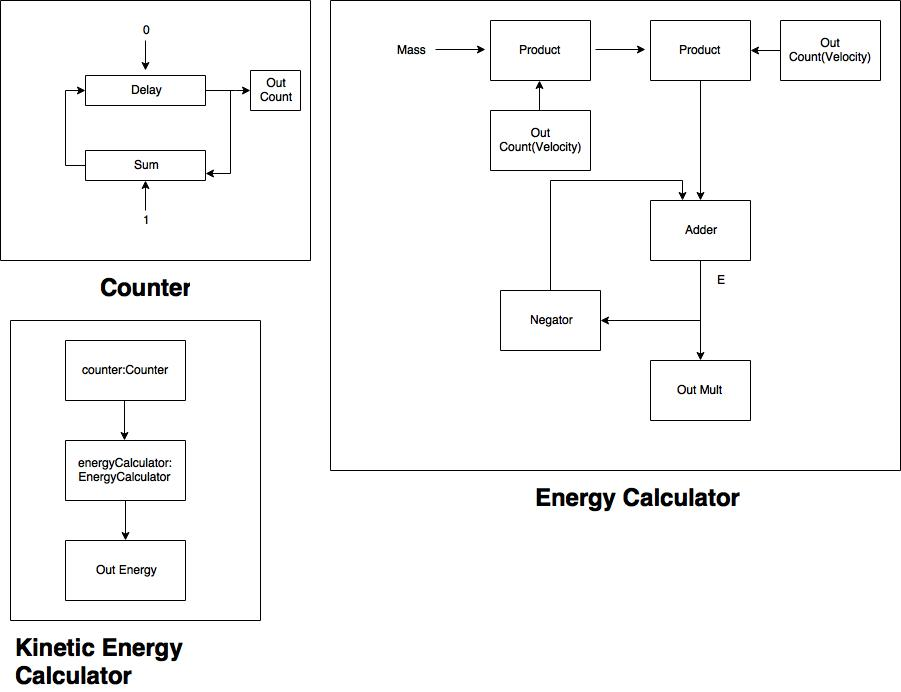
\includegraphics[width = 15cm]{kinetic.jpg}  
\end{figure}
\newpage
\section{Outputs of Kinetic Energy Calculator CBD}
\label{appendix:plot}
\begin{figure}[!ht]
  \centering
  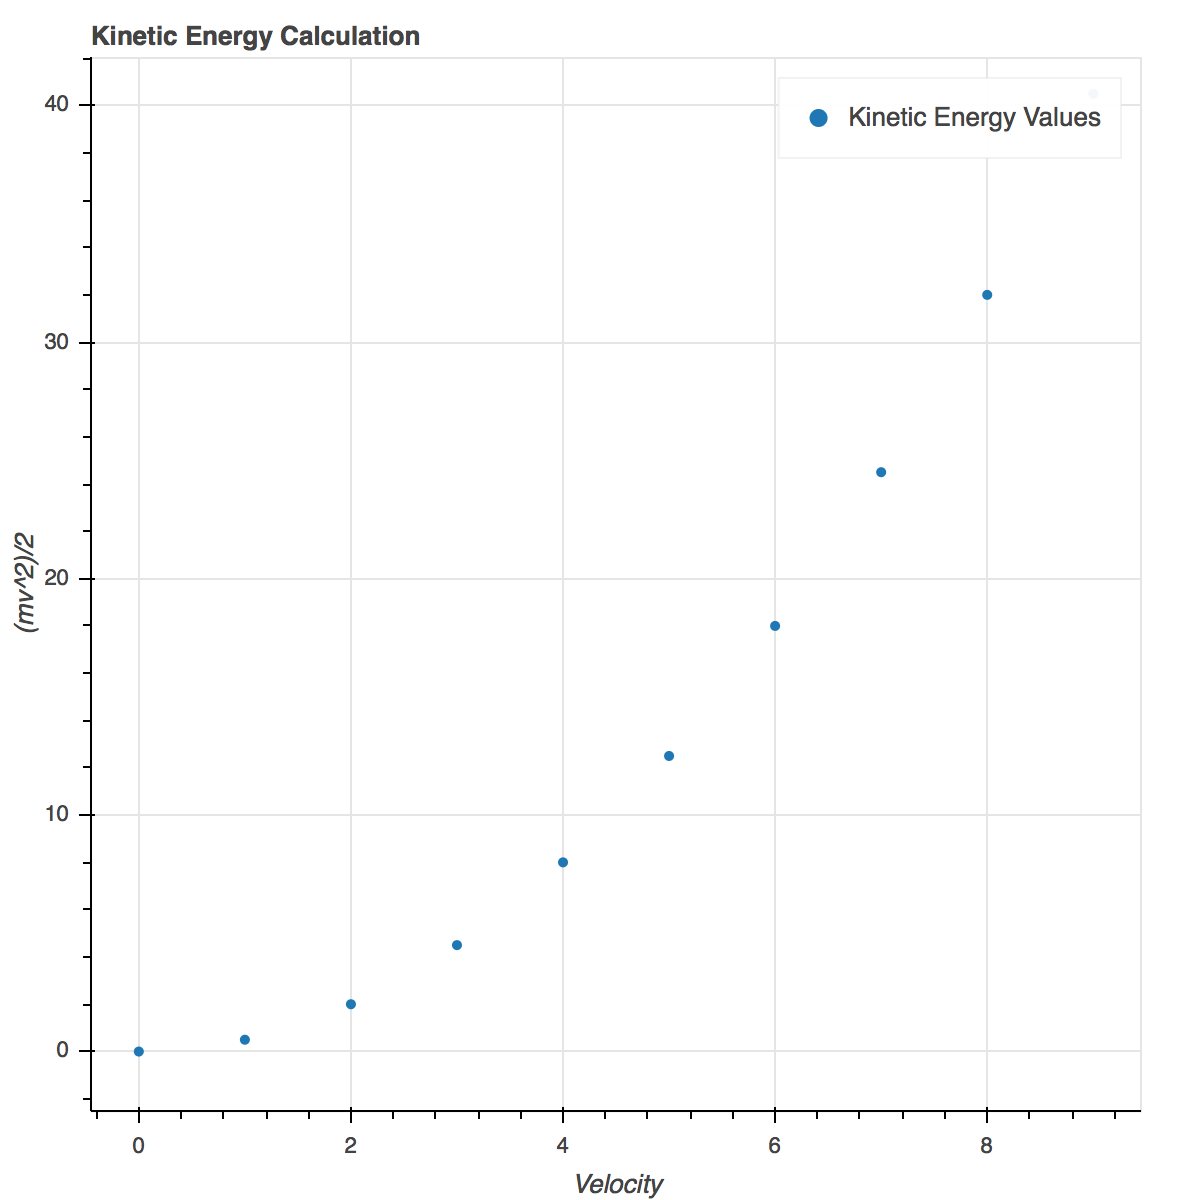
\includegraphics[width = 15cm]{plot.jpg}  
\end{figure}
\newpage
\section{Output denotational semantics CBD}
\label{appendix:oef3}
\(OutEnergy.IN1^{[s+1]} = multiplication.OutMult.OUT1^{[s+1]};\)\\
\(counter.delay.IC^{[s+1]} = counter.zero.OUT1^{[s+1]};\)\\
\(counter.delay.IN1^{[s+1]} = counter.sum.OUT1^{[s+1]};\)\\
\(counter.delay.OUT1^{[s+1]} = counter.delay.IN1^{[s]};\)\\
\(counter.delay.OUT1^{[0]} = counter.delay.IN2^{[0]};\)\\
\(counter.sum.IN1^{[s+1]} = counter.delay.OUT1^{[s+1]};\)\\
\(counter.sum.IN2^{[s+1]} = counter.one.OUT1^{[s+1]};\)\\
\(counter.sum.OUT1^{[s+1]} = counter.sum.IN1^{[s+1]} + counter.sum.IN2^{[s+1]};\)\\
\(counter.zero.OUT1^{[s+1]} = 0.0;\)\\
\(counter.one.OUT1^{[s+1]} = 1.0;\)\\
\(counter.OutCount.IN1^{[s+1]} = counter.delay.OUT1^{[s+1]};\)\\
\(counter.OutCount.OUT1^{[s+1]} = counter.OutCount.IN1^{[s+1]};\)\\
\(multiplication.mult1.IN1^{[s+1]} = multiplication.InNumber.OUT1^{[s+1]};\)\\
\(multiplication.mult1.IN2^{[s+1]} = multiplication.mass.OUT1^{[s+1]};\)\\
\(multiplication.mult1.OUT1^{[s+1]} = multiplication.mult1.IN1^{[s+1]} * multiplication.mult1.IN2^{[s+1]};\)\\
\(multiplication.mult2.IN1^{[s+1]} = multiplication.mult1.OUT1^{[s+1]};\)\\
\(multiplication.mult2.IN2^{[s+1]} = multiplication.InNumber.OUT1^{[s+1]};\)\\
\(multiplication.mult2.OUT1^{[s+1]} = multiplication.mult2.IN1^{[s+1]} * multiplication.mult2.IN2^{[s+1]};\)\\
\(multiplication.mass.OUT1^{[s+1]} = 1.0;\)\\
\(multiplication.adder.IN1^{[s+1]} = multiplication.mult2.OUT1^{[s+1]};\)\\
\(multiplication.adder.IN2^{[s+1]} = multiplication.negator.OUT1^{[s+1]};\)\\
\(multiplication.adder.OUT1^{[s+1]} = multiplication.adder.IN1^{[s+1]} + multiplication.adder.IN2^{[s+1]};\)\\
\(multiplication.negator.IN1^{[s+1]} = multiplication.adder.OUT1^{[s+1]};\)\\
\(multiplication.negator.OUT1^{[s+1]} = -multiplication.negator.IN1^{[s+1]};\)\\
\(multiplication.InNumber.IN1^{[s+1]} = counter.OutCount.OUT1^{[s+1]};\)\\
\(multiplication.InNumber.OUT1^{[s+1]} = multiplication.InNumber.IN1^{[s+1]};\)\\
\(multiplication.OutMult.IN1^{[s+1]} = multiplication.adder.OUT1^{[s+1]};\)\\
\(multiplication.OutMult.OUT1^{[s+1]} = multiplication.OutMult.IN1^{[s+1]};\)\\
\end{appendices}
\end{document}